\section{Zadání}

Pro data v přiloženém souboru odhadněte parametry vybraného nelineárního modelu.
Pro zvolený nelineární model vykreslete konfidenční množinu odhadů a pásy spolehlivosti pro modelované křivky (je možné též zvolit vlastní nelineární model a vlastní data).
Data jsou dostupná v souboru \textit{data05.xlsx}.

\section{Vypracování}

Pro vypracování semestrální práce jsme zvolili data ze čtvrtého listu zadaného excelového souboru.
Tato data byla vygenerována funkcí \( f \).

\begin{equation*}
    f(x, \beta) = \frac{x}{\beta_0 + \beta_1 x^2}
\end{equation*}

\begin{figure}[htb]
    \centering
    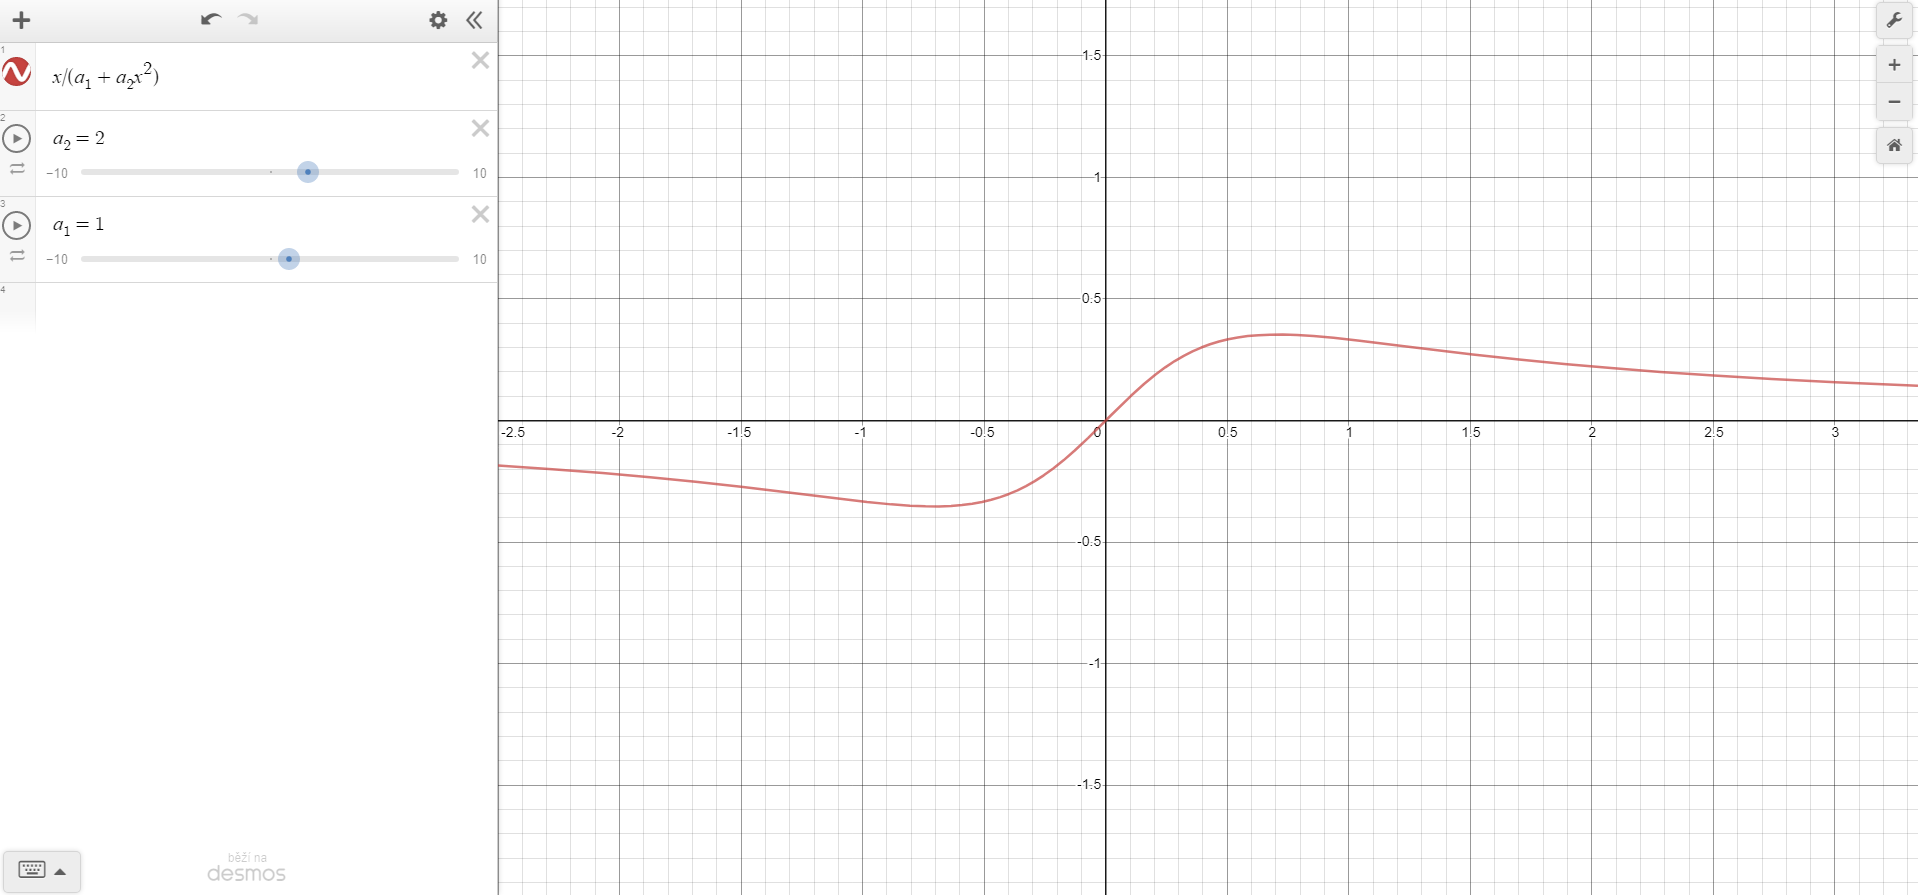
\includegraphics[width=0.95\textwidth]{graphs/desmos.png}
    \caption{Náhled funkce použité k vygenerování dat v prostředí Desmos}
    \label{fig:lr1}
\end{figure}
\FloatBarrier

Při odhadu parametrů \( \beta \) jsme zvolili 2 přístupy.
Prvním přístupem je přímá linearizace modelu.
Výsledné hodnoty jsou vidět na grafu~\ref{fig:lr2}.
V našem případě nedává metoda přímé linearizace dostatečně dobré výsledky, vygenerovaná data se příliš odchylují od dat původních.

\begin{figure}[htb]
    \centering
    \vspace*{0in}

    \begin{equation*}
        \beta = \left[ \begin{matrix} -13.5584 \\ 9.7383 \end{matrix} \right]
    \end{equation*}

    \label{eq:linear}
    \caption{Odhady koeficientů metodou linearizace}
\end{figure}
\FloatBarrier

Zvolili jsme tedy druhou metodu odhadu parametrů – pomocí nelineární regrese.
Tato metoda funguje dle očekávání dobře, výsledek je k nahlédnutí v grafu~\ref{fig:lr2}.

\begin{figure}[htb]
    \centering
    \vspace*{0in}

    \begin{equation*}
        \beta = \left[ \begin{matrix} 2.0077 \\ 0.9950 \end{matrix} \right]
    \end{equation*}

    \label{eq:linear}
    \caption{Odhady koeficientů metodou nelineární regrese}
\end{figure}
\FloatBarrier

\begin{figure}[htb]
    \centering
    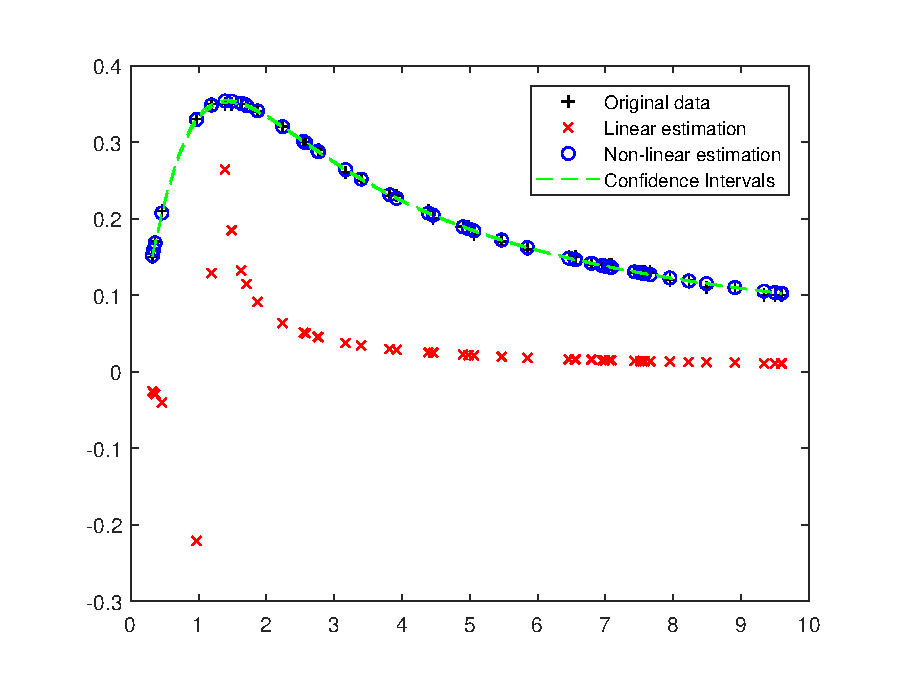
\includegraphics[width=0.7\textwidth]{graphs/fig1.eps}
    \caption{Data a jejch funkční odhady}
    \label{fig:lr2}
\end{figure}
\FloatBarrier

Druhou částí zadání je nalezení a vykreslení \( 95 \% \) intervalů spolehlivosti.
Pro jejich výpočet byly použity koeficienty \( \beta \) vypočtené metodou nelineární regrese, jakožto nejlepší odhad.
Výsledky jsou vidět na grafu~\ref{fig:lr2}, detail pak na grafu~\ref{fig:lr3}.

\begin{figure}[htb]
    \centering
    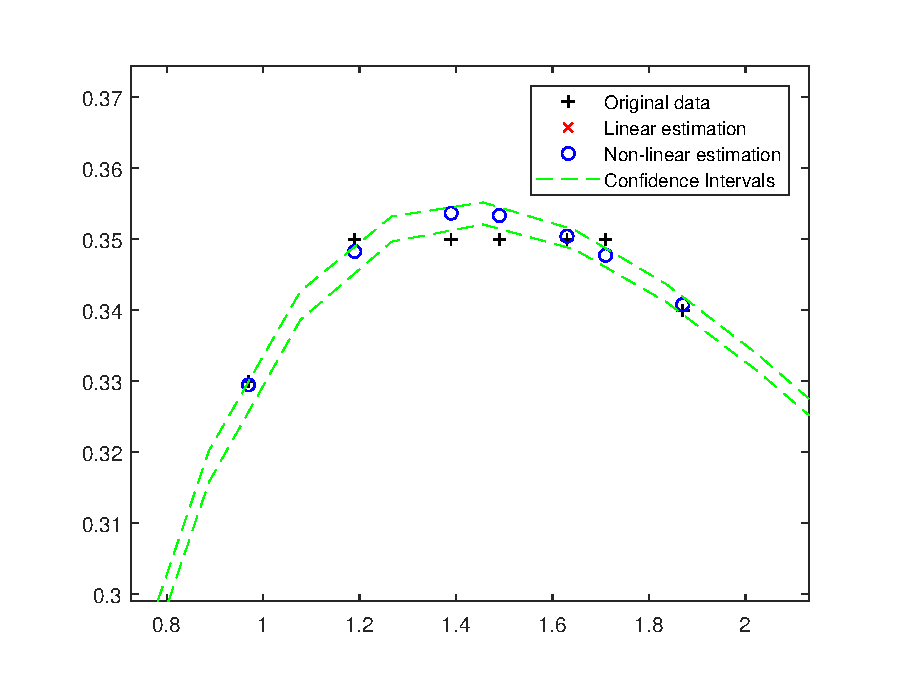
\includegraphics[width=0.55\textwidth]{graphs/fig2.eps}
    \caption{Intervaly spolehlivosti}
    \label{fig:lr3}
\end{figure}
\FloatBarrier

\section{Závěr}

V semestrální práci odhadovali parametry nelineárního modelu dvěma odlišnými přístupy.
Získali jsme představu o využitelnosti a přesnosti obou metod.

V druhé části práce jsme získávali intervaly spolehlivosti.
Jejich využití je především v úlohách obsahujících náhodnou složku, nám však jejich výpočet a vykreslení dokázali správnost odhadnutých parametrů.
Obecně lze označit získané výsledky za uspokojivé.
